\section{分布的定义与例子}

参见于品数学分析讲义

\subsection{试验函数}

我们用 $\mathcal{D}(\Omega)=C_0^{\infty}(\Omega)$ 表示在 $\Omega$ 上定义并且有紧支集的光滑函数所组成的集合,我们把它称作是为试验函数空间。按照定义,对于任意的 $\varphi \in \mathcal{D}(\Omega)$ ,存在紧集 $K \subset \Omega$(这是 $\mathbb{R}^n$ 中的紧集),使得 $\left.f\right|_{\Omega-K} \equiv 0$ ,即对任意的 $x \in \Omega-K, f(x)=0$ 。

\subsubsection{试验函数的闭包}

以下是一些常见的闭包及其对应的函数空间:

\begin{enumerate}
	\item 在 $L^p(\Omega)$ 空间中(使用 $L^p$ 范数):
\end{enumerate}

试验函数空间 $\mathcal{D}(\Omega)$ 在 $L^p(\Omega)$ 空间中是稠密的,对于 $1 \leq p<\infty$。这意味着 $\mathcal{D}(\Omega)$ 在 $L^p$ 范数下的闭包是整个 $L^p(\Omega)$ 空间。

简单来说,任何一个 $L^p$ 函数都可以通过一列试验函数在该范数下逼近。

\begin{enumerate}
	\item 在连续函数空间 $C(\Omega)$ 或 $C_b(\Omega)$ 中(使用一致范数 $\|f\|_{\infty}$):
\end{enumerate}

试验函数是连续的,并且具有紧支集。在一致范数下,试验函数空间 $\mathcal{D}(\Omega)$ 的闭包是具有紧支集的连续函数空间 $C_c(\Omega)$。这是因为任何一个紧支集连续函数都可以通过光滑的,紧支集函数(例如通过卷积光滑化)来一致逼近。

\begin{enumerate}
	\item 在 Sobolev 空间 $W^{k, p}(\Omega)$ 中(使用 Sobolev 范数):
\end{enumerate}

试验函数空间 $\mathcal{D}(\Omega)$ 在 Sobolev 空间 $W^{k, p}(\Omega)$ 中是稠密的,对于 $1 \leq p<\infty$ 和非负整数 $k \geq 0$。这意味着 $\mathcal{D}(\Omega)$ 在 $W^{k, p}$ 范数下的闭包是整个 Sobolev 空间 $W^{k, p}(\Omega)$。Sobolev 空间是研究偏微分方程非常重要的函数空间,它包含了直到 $k$ 阶的广义导数(或弱导数)存在且属于 $L^p$ 空间的函数。

\subsection{分布}

\begin{definition}[分布]
所谓$\Omega$ 上的一个\textbf{分布}(也称作广义函数)指的是 $\mathcal{D}(\Omega)$ 上的一个线性泛函(线性映射):
\[
u: \mathcal{D}(\Omega) \rightarrow \mathbb{C}, \quad \varphi \mapsto\langle u, \varphi\rangle
\]满足如下两个条件
	\begin{enumerate}
		\item 对任意的$\varphi, \psi \in \mathcal{D}(\Omega)$ 和 $\alpha, \beta \in \mathbb{C}$ ,我们有
	\end{enumerate}
\[
\langle u, \alpha \varphi+\beta \psi\rangle=\alpha\langle u, \varphi\rangle+\beta\langle u, \psi\rangle .
\]	\begin{enumerate}
		\item 对任意的紧集$K \subset \Omega$,存在非负整数$p$ 和正常数$C$($p$ 和$C$ 依赖于$K$),使得对任意的$\varphi \in C_K^{\infty}(\Omega)$,都有
	\end{enumerate}
\[
|\langle u, \varphi\rangle| \leqslant C \sup _{|\alpha| \leqslant p}\left\|\partial^\alpha \varphi\right\|_{L^{\infty}(K)}
\]如果上述的 $p$ 的选取不依赖于紧集 $K$ 的选取,那么,我们就把最小的这样的非负整数 $p$ 称作是分布 $u$ 的阶。\label{1d3091}
\end{definition}

\begin{example}
对任意的 $a \in \Omega$,我们可以定义分布 $\delta_a \in \mathcal{D}^{\prime}(\Omega)$。其中,对于任意的 $\varphi \in \mathcal{D}(\Omega)$,我们定义
\[
\left\langle\delta_a, \varphi\right\rangle=\varphi(a)
\]我们来验证 $\delta_a$ 实际上是分布:
对任意的紧集 $K \subset \Omega$,如果 $a \notin K$,那么,对任意的 $\varphi \in C_K^{\infty}(\Omega)$,我们都有
\[
\left\langle\delta_a, \varphi\right\rangle=0
\]如果 $a \in K$,那么,使得对任意的 $\varphi \in C_K^{\infty}(\Omega)$,我们有
\[
\left|\left\langle\delta_a, \varphi\right\rangle\right|=|\varphi(a)| \leqslant 1 \cdot \sup _{|\alpha| \leqslant 0}\left\|\partial^\alpha \varphi\right\|_{L^{\infty}(K)} .
\]所以,我们在分布的定义中取 $q=0, C=1$ 即可。特别地,我们还知道 $\delta_a$ 的阶为 0。
\end{example}
\begin{example}
给定开集 $\Omega$(总是装配了 Borel 代数和 Lebesgue 测度),\textbf{局部可积的函数}指的是在每个紧的局部上都可积的函数,即可测函数 $f$(所对应的几乎处处相等的函数的等价类),对于任意紧集 $K \subset \Omega$,函数 $f \cdot \mathbf{1}_K \in L^1(\Omega)$。我们用 $L_{\mathrm{loc}}^1(\Omega)$ 表示 $\Omega$ 上局部可积的函数。
对于任意的 $f \in L_{\mathrm{loc}}^1(\Omega)$,我们定义 $\mathcal{D}(\Omega)$ 上的线性泛函:
\[
T_f: \mathcal{D}(\Omega) \rightarrow \mathbb{C}, \varphi \mapsto\left\langle T_f, \varphi\right\rangle=\int_{\Omega} f(x) \varphi(x) d x
\]由于 $\varphi$ 在它的支集 $K$ 上有界,所以,上面的积分是良好定义的。我们证明 $T_f$ 是 $\Omega$ 上的阶为 0 的分布:对任意的紧集 $K \subset \Omega$,对任意的 $\varphi \in C_K^{\infty}(\Omega)$,我们有
\[
\begin{aligned}
\left|\left\langle T_f, \varphi\right\rangle\right| & =\left|\int_K f(x) \varphi(x) d x\right| \\
& \leqslant\|f\|_{L^1(K)}\|\varphi\|_{L^{\infty}(K)} .
\end{aligned}
\]所以,我们在分布的定义中取 $q=0,\|f\|_{L^1(K)}$ 即可.
\end{example}
\begin{remark}
为了方便起见,我们通常把 $\left\langle T_f, \varphi\right\rangle$ 直接写成 $\langle f, \varphi\rangle$。
\end{remark}
\begin{proposition}
任意选定 $\chi(x) \in \mathcal{D}\left(\mathbb{R}^n\right)$(我们通常偏爱之前所构造的那个 $\chi(x)$ ),我们假定
\[
\int_{\mathbb{R}^n} \chi(x) d x=1
\]对任意的 $\varepsilon>0$ ,我们定义
\[
\chi_{\varepsilon}(x)=\frac{1}{\varepsilon^n} \chi\left(\frac{x}{\varepsilon}\right) .
\]那么,在分布的意义下,当 $\varepsilon \rightarrow 0$ 时,我们有 $\chi_{\varepsilon} \xrightarrow{\mathcal{D}^{\prime}} \delta_0$ 。
\end{proposition}
\begin{example}
假设 $\mu$ 是 $(\Omega, \mathcal{B}(\Omega))$ 上的测度,其中,$\Omega \subset \mathbb{R}^n$ 是开集,$\mathcal{B}(\Omega)$ 是 Borel 代数(包含所有开集的最小 $\sigma$-代数)。如果每个紧集 $K \subset \Omega, \mu(K)<\infty$,我们就把这种测度称作是一个 \textbf{Radon 测度}。
比如说,对任意的正函数(几乎处处)$f \in L_{\mathrm{loc}}^1(\Omega)$,对任意的 $B \in \mathcal{B}(\Omega)$,我们可以定义
\[
\mu_f(B)=\int_{\Omega} \mathbf{1}_B \cdot f(x) d x
\]这就是一个 Radon 测度。
任意给定一个 Radon 测度 $\mu$,我们可以定义一个分布 $T_\mu$:对于 $\varphi \in \mathcal{D}(\Omega)$,我们要求
\[
\left\langle T_\mu, \varphi\right\rangle=\int_{\Omega} \varphi(x) d \mu(x)
\]我们证明 $T_\mu$ 是 $\Omega$ 上阶为 0 的分布:
对任意的紧集 $K \subset \Omega$,对任意的 $\varphi \in C_K^{\infty}(\Omega)$,我们有
\[
\begin{aligned}
\left|\left\langle T_\mu, \varphi\right\rangle\right| & =\left|\int_K \varphi(x) d \mu(x)\right| \\
 & \leqslant \mu(K)\|\varphi\|_{L^{\infty}(K)}
\end{aligned}
\]所以,我们在分布的定义中取 $q=0, C=\mu(K)$ 即可。
特别地,我们可以把 $L_{\mathrm{loc}}^1(\Omega)$ 中的元素看作是某个 Radon 测度的密度函数,从而,定义出了同样的分布。
\end{example}
\begin{remark}
利用所谓的 Riesz 表示定理,我们可以证明,$\Omega$ 上所有的 0 阶分布都是(由如上方式给出的)Radon 测度。
\end{remark}
\begin{proposition}
给定开集 $\Omega \subset \mathbb{R}^n$,我们已经定义如下的线性映射(把局部可积函数视为分布)
\[
T: L_{\mathrm{loc}}^1(\Omega) \rightarrow \mathcal{D}^{\prime}(\Omega), \quad f \mapsto T_f
\]这是单射。
\end{proposition}
\begin{remark}
根据这个命题,局部可积的函数可以看做是分布的子集合。在分析中,我们把 $L_{\mathrm{loc}}^1(\Omega)$ 的元素称作是 $\Omega$ 上的“函数”(这个类已经足够大了),由于某些分布不是“函数”,所以我们也经常把分布称作是“广义函数”。
\end{remark}
\begin{lemma}
假设 $\psi(x) \in C^{\infty}(\mathbb{R})$ 并且 $\psi(0)=0$,那么,$\frac{\psi(x)}{x}$ 也是光滑函数。
\end{lemma}
所以 $\frac{\varphi(x)-\varphi(-x)}{x}$ 是光滑函数(自然是局部可积的)。从而,当 $n \rightarrow \infty$ 时,上述积分的极限存在:
\[
\lim _{n \rightarrow \infty} \int_{\frac{1}{n}}^{\infty} \frac{\varphi(x)-\varphi(-x)}{x} d x=\int_0^{\infty} \frac{\varphi(x)-\varphi(-x)}{x} d x
\]
我们现在定义
\[
\left\langle\operatorname{vp} \frac{1}{x}, \varphi\right\rangle=\int_0^{\infty} \frac{\varphi(x)-\varphi(-x)}{x} d x
\]
为了证明这是分布,我们利用中值定理:对任意的紧集 $K=[-M, M] \subset \mathbb{R}$ ,对任意的支集在 $K$ 上的光滑函数 $\varphi$ ,我们有
\[
|\varphi(x)-\varphi(-x)|=\left|2 x \varphi^{\prime}(\xi)\right| \leqslant 2\left\|\varphi^{\prime}\right\|_{L^{\infty}(K)} x
\]
所以,
\[
\left|\left\langle\operatorname{vp} \frac{1}{x}, \varphi\right\rangle\right| \leqslant \int_0^M 2\left\|\varphi^{\prime}\right\|_{L^{\infty}(K)} d x=2 M\left\|\varphi^{\prime}\right\|_{L^{\infty}(K)}
\]
所以 $\operatorname{vp} \frac{1}{x}$ 是一个阶不超过 1 的分布。在作业中,我们将证明 $\operatorname{vp} \frac{1}{x}$ 的阶恰好是 1 。

\begin{note}
另外,vp 是法语 valeur principale 的缩略,英文文献经常用 $\mathrm{pv} \frac{1}{x}$ ,因为他们把主值写为 principal value。
\end{note}
\section{分布的操作:限制,求导数,与微分同胚复合,链式法则。Stokes 公式的分布形式。}

在微积分的学习中,我们可以对一个函数做特定的操作,比如可以把一个函数限制到比较小的定义域上、可以对一个函数求导数、两个函数可以相乘等等。我们现在讨论如何对分布做一些特定的操作。

\begin{note}
我们通常用 $\varphi$ 表示试验函数.
\end{note}
\subsection{分布的限制}

假设 $\Omega^{\prime} \subset \Omega$ 是开子集,那么,我们可以定义限制映射
\[
\operatorname{Res} : \mathcal{D}^{\prime}(\Omega) \rightarrow \mathcal{D}^{\prime}\left(\Omega^{\prime}\right), u \mapsto \operatorname{Res}(u) .
\]
其中,对于每个 $\varphi \in \mathcal{D}\left(\Omega^{\prime}\right)$ ,它自然可以看作是 $\mathcal{D}(\Omega)$ 中的元素,从而,我们可以要求
\[
\langle\operatorname{Res}(u), \varphi\rangle=\langle u, \varphi\rangle .
\]
\subsection{求偏导数}

通过分部积分,我们有
\[
\begin{aligned}
\left\langle u^{\prime}, \varphi\right\rangle & =\int_{\mathbb{R}} u^{\prime}(x) \varphi(x) d x=-\int_{\mathbb{R}} u(x) \varphi^{\prime}(x) d x \\
& =-\left\langle u, \varphi^{\prime}\right\rangle .
\end{aligned}
\]
这个计算启发我们对于 $u \in \mathcal{D}^{\prime}(\mathbb{R})$ ,我们可以用下面的等式来定义它的导数:
\[
\left\langle u^{\prime}, \varphi\right\rangle:=-\left\langle u, \varphi^{\prime}\right\rangle .
\]
\begin{definition}
假设 $\Omega \subset \mathbb{R}^n$ 是有界开集,给定 $u \in \mathcal{D}^{\prime}(\Omega)$ ,对于任意的多重指标 $\alpha$ ,我们\textbf{定义}
\[
\left\langle\partial^\alpha u, \varphi\right\rangle=(-1)^{|\alpha|}\left\langle u, \partial^\alpha \varphi\right\rangle .
\]
\end{definition}
显然根据分布的定义,\cref{1d3091},第二条,可知分布的导数依然是分布。

\begin{example}
我们计算 $\mathbb{R}$ 上的 Dirac 函数 $\delta_a$ 的导数,其中 $a \in \mathbb{R}$ 。任给 $\varphi \in \mathcal{D}(\mathbb{R})$ ,我们有
\[
\left\langle\delta_a^{\prime}, \varphi\right\rangle=-\left\langle\delta_a, \varphi^{\prime}\right\rangle=-\varphi^{\prime}(a) .
\]
\end{example}
\subsection{\texorpdfstring{$C^{\infty}(\Omega)$}{C^infty(Omega)} -模结构}

对光滑函数 $f \in C^{\infty}(\Omega)$ 和分布 $u \in \mathcal{D}^{\prime}(\Omega)$ ,我们可以定义它们的乘积 $f \cdot u$:
\[
\langle f \cdot u, \varphi\rangle:=\langle u, f \varphi\rangle .
\]
下一步验证 $f\cdot u\in \mathcal{D}'(\Omega)$,进而分布具有 $C^{\infty}(\Omega)$ -模结构.
\[
|\langle f \cdot u, \varphi\rangle| \leqslant C \sup _{|\alpha| \leqslant p}\left\|\partial^\alpha(f \cdot \varphi)\right\|_{L^{\infty}(K)}
\]
根据 Leibniz 法则,我们有
\[
\partial^\alpha(f \cdot \varphi)=\sum_{\beta+\gamma=\alpha} \partial^\beta f \cdot \partial^\gamma \varphi
\]
所以,
\[
\begin{aligned}
|\langle f \cdot u, \varphi\rangle| \leqslant & C \sup _{|\alpha| \leqslant p} \sum_{\beta+\gamma=\alpha}\left\|\partial^\beta f\right\|_{L^{\infty}(K)}\left\|\partial^\gamma \varphi\right\|_{L^{\infty}(K)} \\
& \leqslant \underbrace{C \sum_{|\beta| \leqslant p}\left\|\partial^\beta f\right\|_{L^{\infty}(K)}}_{\text {新的常数 } C^{\prime}} \times \sup _{|\gamma| \leqslant p}\left\|\partial^\gamma \varphi\right\|_{L^{\infty}(K)}
\end{aligned}
\]
这表明 $f \cdot u \in \mathcal{D}^{\prime}(\Omega)$。

\subsection{分布的平移和变量替换}

对于 $x_0 \in \mathbb{R}^n$ ,我们有如下的平移变换:
\[
\tau_{x_0}: \mathbb{R}^n \rightarrow \mathbb{R}^n, \quad x \mapsto x+x_0 .
\]
对于局部可积的函数 $f \in L_{\mathrm{loc}}^1\left(\mathbb{R}^n\right)$ ,我们可以定义(这是一种特殊的变量替换):
\[
(\tau_{x_0}f)(x)\coloneqq (f\circ \tau_{x_0})(x)=f(x+x_0)
\]
对一般的分布 $u\in \mathcal{D}'(\mathbb{R}^{n})$, $x_0\in \mathbb{R}^{n}$,我们定义
\[
\left< \tau_{x_0}u,\varphi \right> \coloneqq  \left< u,\varphi(x-x_0) \right>
\]
容易验证 $\tau_{x_0}u\in \mathcal{D}'(x_0)$. (承自上一节中分布的 $C^{\infty}(\Omega)$ -模结构)

给定$\mathbb{R}^n$的两个开集$\Omega_1$和$\Omega_2$,我们假定
\[
\Phi: \Omega_1 \rightarrow \Omega_2
\]
是微分同胚。对任意一个$\Omega_2$上的局部可积的函数$f$和$\Omega_1$上的试验函数$\varphi$,根据换元积分公式,我们有
\[
\begin{aligned}
\left\langle\Phi^* f, \varphi(x)\right\rangle & =\int_{\Omega_1} f(\Phi(x)) \varphi(x) d x=\int_{\Omega_2} f(y) \varphi\left(\Phi^{-1}(y)\right)\left|\mathbf{J}_{\Phi^{-1}}(y)\right| d y \\
& =\int_{\Omega_2} f(y) \frac{\varphi\left(\Phi^{-1}(y)\right)}{\left|\mathbf{J}_{\Phi}\left(\Phi^{-1}(y)\right)\right|} d y \\
& =\left\langle f, \frac{\varphi\left(\Phi^{-1}(y)\right)}{\left|\mathbf{J}_{\Phi}\left(\Phi^{-1}(y)\right)\right|}\right\rangle .
\end{aligned}
\]
根据这个计算,我们定义:
\[
\Phi^*: \mathcal{D}^{\prime}\left(\Omega_2\right) \rightarrow \mathcal{D}^{\prime}\left(\Omega_1\right), \quad u \mapsto \Phi^* u .
\]
其中,对于$u \in \mathcal{D}^{\prime}\left(\Omega_2\right)$和$\varphi \in \mathcal{D}\left(\Omega_1\right)$,对于我们定义$\Phi^* u$如下:
\[
\left\langle\Phi^* u, \varphi(x)\right\rangle:=\left\langle u, \varphi\left(\Phi^{-1}(y)\right)\left|\mathbf{J}_{\Phi^{-1}}(y)\right|\right\rangle=\left\langle u, \frac{\varphi\left(\Phi^{-1}(y)\right)}{\left|\mathbf{J}_{\Phi}\left(\Phi^{-1}(y)\right)\right|}\right\rangle .
\]
简单验证可知:$\Phi^{*}u\in \mathcal{D}'(\Omega)$.

\begin{remark}
注记(记号).因为在光滑函数情况下,$\Phi^* u$ 就是函数的复合,我们还把上面的拉回映射写成
\[
u \circ \Phi=\Phi^* u .
\]
\end{remark}
给定微分同胚 $\Phi: \Omega_1 \rightarrow \Omega_2$,它把 $\Omega_2$ 上的 Dirac 函数拉回,得到 $\Omega_1$ 上的 Dirac 函数,这给出了 Jacobi 行列式的一个精确的解释:这是一点处体积的变化。

\subsubsection{链式法则}

给定微分同胚 $\Phi$ ,如果 $u$ 是 $C^1$ 的函数,我们可以对求导数运算运用链式法则:
\[
\partial_j(u \circ \Phi)=\sum_{k=1}^n \partial_j \Phi_k\left(x_1, \cdots, x_n\right) \cdot\left(\partial_k u \circ \Phi\right)\left(x_1, \cdots, x_n\right) .
\]
对于一般的分布 $u$ ,我们实际上(后来)可以先用光滑函数逼近这个分布,然后上面的链式法则在极限的情况下仍然成立。

我们现在给出一个直接的证明:设 $\Psi=\Phi^{-1}$ 是 $\Phi$ 的逆映射。按照分布与一个微分同胚的复合的定义,我们有
\[
\begin{aligned}
\left\langle\sum_{k=1}^n \frac{\partial \Phi_k}{\partial x_j} \cdot \frac{\partial u}{\partial y_k} \circ \Phi, \varphi\right\rangle & =\sum_{k=1}^n\left\langle\frac{\partial u}{\partial y_k} \circ \Phi, \frac{\partial \Phi_k}{\partial x_j} \cdot \varphi\right\rangle \\
& =\sum_{k=1}^n\left\langle\frac{\partial u}{\partial y_k},\left(\frac{\partial \Phi_k}{\partial x_j} \circ \Psi\right)(\varphi \circ \Psi)\right| J_{\Psi}| \rangle \\
& =-\sum_{k=1}^n\left\langle u, \frac{\partial}{\partial y_k}\left[\left(\frac{\partial \Phi_k}{\partial x_j} \circ \Psi\right)(\varphi \circ \Psi)\left|J_{\Psi}\right|\right]\right\rangle
\end{aligned}
\]
另外,对任意 $g \in C_0^{\infty}(\Omega)$ ,我们有
\[
\begin{aligned}
0 & =\int_{\Omega_1} \frac{\partial}{\partial x_j}(g \circ \Phi) d x=\sum_{k=1}^n \int_{\Omega_1} \frac{\partial \Phi_k}{\partial x_j} \cdot \frac{\partial g}{\partial y_k} \circ \Phi \\
& =\sum_{k=1}^n \int_{\Omega_2} \frac{\partial \Phi_k}{\partial x_j} \circ \Psi \cdot \frac{\partial g}{\partial y_k} \cdot\left|\mathbf{J}_{\Psi}(y)\right| d y \\
& =-\sum_{k=1}^n \int_{\Omega_2} g \frac{\partial}{\partial y_k}\left(\frac{\partial \Phi_k}{\partial x_j} \circ \Psi \cdot\left|\mathbf{J}_{\Psi}(y)\right|\right) d y
\end{aligned}
\]
根据 $L_{\mathrm{loc}}^1(\Omega)$ 到 $\mathcal{D}^{\prime}(\Omega)$ 嵌入的单射性,上面的等式等价于说
\[
\sum_{k=1}^n \frac{\partial}{\partial y_k}\left(\frac{\partial \Phi_k}{\partial x_j} \circ \Psi \cdot\left|\mathbf{J}_{\Psi}(y)\right|\right)=0
\]
从而
\[
\begin{aligned}
\left\langle\sum_{k=1}^n \frac{\partial \Phi_k}{\partial x_j} \cdot \frac{\partial u}{\partial y_k} \circ \Phi, \varphi\right\rangle & =-\sum_{k=1}^n\left\langle u, \frac{\partial}{\partial y_k}(\varphi \circ \Psi)\left[\left(\frac{\partial \Phi_k}{\partial x_j} \circ \Psi\right)\left|\mathbf{J}_{\Psi}\right|\right]\right\rangle \\
& =\left\langle u, \frac{\partial \varphi}{\partial x_j} \circ \Psi\right| \mathbf{J}_{\Psi}| \rangle \\
& =-\left\langle u \circ \Phi, \frac{\partial \varphi}{\partial x_j}\right\rangle
\end{aligned}
\]
这就证明如下关于分布的链式法则:
\[
\partial_j\left(\Phi^* u\right)=\sum_{k=1}^n \partial_j \Phi_k \cdot \Phi^*\left(\left(\partial_k u\right)\right) .
\]
\subsection{关于分布的 Stokes 公式}

\begin{theorem}
(Stokes 公式) 假设$\Omega$ 是一个有界带边光滑区域,$\nu(x)=\left(\nu_1(x), \cdots, \nu_n(x)\right)$ 为 $\partial \Omega$ 的单位外法向量,$d \sigma$ 为 $\partial \Omega$ 上的曲面测度。对任意的 $\varphi \in C^1\left(\mathbb{R}^n, \mathbb{C}\right)$ ,我们有
\[
\int_{\Omega} \frac{\partial \varphi}{\partial x_i}(x) d x=\int_{\partial \Omega} \varphi(x) \nu_i(x) d \sigma
\]
\end{theorem}
\begin{figure}[H]
\centering
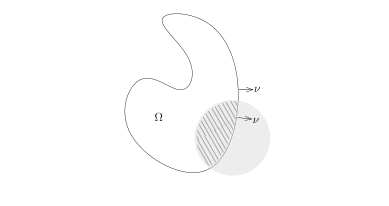
\includegraphics[width=\textwidth]{2-分布-2025050221.png}
% \caption{}
\label{}
\end{figure}

给定上面 Stokes 公式中所述的 $\Omega$,它的边界 $\partial \Omega$ 的曲面测度 $d \sigma$ 在如下的意义下定义了 $\mathbb{R}^n$ 上一个分布:
\[
d \sigma: \mathcal{D}\left(\mathbb{R}^n\right) \rightarrow \mathbb{C}, \quad \varphi \mapsto \int_{\partial \Omega} \varphi(x) d \sigma(x)
\]
这是一个 0 阶的分布,我们把证明的细节留给不放心的同学来验证。类似地,对每一个 $i \leqslant n$,如下的公式也定义了一个分布:
\[
\nu_i d \sigma: \mathcal{D}\left(\mathbb{R}^n\right) \rightarrow \mathbb{C}, \quad \varphi \mapsto \int_{\partial \Omega} \varphi(x) \nu_i(x) d \sigma(x)
\]
我们可以把 Stokes 公式改写成如下的形式:
\[
\left\langle\mathbf{1}_{\Omega}, \partial_i \varphi\right\rangle=\int_{\mathbb{R}^n} \mathbf{1}_{\Omega}(x) \frac{\partial \varphi}{\partial x_i}(x) d x=\int_{\partial \Omega} \varphi(x) \nu_i(x) d \sigma .
\]
所以,用分布的语言来写,我们有

\begin{theorem}[Stokes 公式]
假设 $\Omega$ 是一个有界带边光滑区域,$\nu(x)=\left(\nu_1(x), \cdots, \nu_n(x)\right)$ 为 $\partial \Omega$ 的单位外法向量,$d \sigma$ 为 $\partial \Omega$ 上的曲面测度,作为分布,我们有等式
\[
\partial_i \mathbf{1}_{\Omega} \stackrel{\mathcal{D}^{\prime}\left(\mathbb{R}^n\right)}{=}-\nu_i d \sigma .
\]如果用向量值分布的语言(可以望文生义地定义)来写,我们有
\[
\nabla \mathbf{1}_{\Omega} \stackrel{\mathcal{D}^{\prime}\left(\mathbb{R}^n\right)}{=}-\nu d \sigma .
\]
\end{theorem}
我们现在回到 1 维的情形,此时的 Stokes 公式就是 Newton-Leibniz 公式。

\begin{lemma}
对于 $f(x) \in L^1((a, b))$ ,我们定义其原函数为
\[
F(x)=\int_a^x f(y) d y .
\]那么,$F(x)$ 是连续函数。在分布的意义下,我们有
\[
F(x)^{\prime} \stackrel{\mathcal{D}^{\prime}}{=} f(x) .
\]
\end{lemma}
证明只需照章办事.(利用 Fubini 定理)

\section{分布的应用}

这里跳过第 60 节

\section{分布的局部刻画}

\subsection{单位分解定理}

\begin{theorem}[单位分解]
任意给定$\mathbb{R}^n$ 中的紧集 $K$ ,假设 $K$ 被有限个开集 $\left\{U_1, \cdots, U_N\right\}$ 所覆盖。那么,对每个 $j \leqslant N$ ,存在光滑函数 $\chi_j \in C_0^{\infty}\left(U_j\right)$ ,满足
	\begin{enumerate}
		\item 对任意 $x \in \mathbb{R}^n$ ,有 $0 \leqslant \chi_j(x) \leqslant 1$ ;
		\item 存在包含 $K$ 的开集 $V$ ,对任意 $x \in V$ ,我们有
	\end{enumerate}
\[
\chi_1(x)+\cdots+\chi_N(x)=1 .
\]
\end{theorem}
\begin{note}
单位分解的证明并没有任何启发性的意义,我们只要能够运用该结论即可。
\end{note}
我们现在证明一个分布 $u$ 在(所有)小的开集上的限制决定了 $u$,这表明分布是可以局部定义的:

\begin{theorem}
给定开集 $\Omega \subset \mathbb{R}^n$。任意给定一族开集 $\left\{\Omega_i \mid i \in I\right\}$,其中对任意的 $i \in I, \Omega_i \subset \Omega$。我们假定
\[
\Omega=\bigcup_{i \in I} \Omega_i
\]对每个 $i \in I$,我们在 $\Omega_i$ 上指定一个分布 $u_i \in \mathcal{D}^{\prime}\left(\Omega_i\right)$。如果这一族分布 $\left\{u_i\right\}_{i \in I}$ 满足如下的相容关系:
\[
\left.u_i\right|_{\Omega_i \cap \Omega_j}=\left.u_j\right|_{\Omega_i \cap \Omega_j}, \quad \text { 对任意的 } i, j \in I \text {, }
\]那么,存在唯一的 $u \in \mathcal{D}^{\prime}(\Omega)$,使得对任意的 $i \in I$,我们都有
\[
\left.u\right|_{\Omega_i}=u_i
\]进一步,$u \in L_{\mathrm{loc}}^1(\Omega)$ 当且仅当对每个 $i \in I,\left. u\right|_{\Omega_i} \in L_{\mathrm{loc}}^1 (\Omega)$; $u \in C^k(\Omega)$ 当且仅当对每个 $i \in I$,$\left.u\right|_{\Omega_i} \in C^k(\Omega)$,其中 $k \in \mathbb{Z}_{\geqslant 0}$。
\end{theorem}
\begin{note}
这个定理表明,在 $\mathbb{R}^n$ 的开集上所定义的分布可以构成 $\mathbb{R}^n$ 上的一个\textbf{层}。
\end{note}
\subsubsection{层}

在代数几何中,仿射空间$\mathbb{R}^n$上的层通常指的是在某个拓扑空间(比如$\mathbb{R}^n$赋予通常的欧几里得拓扑)上的一个结构,它将每个开集关联到一个代数对象(比如一个环、一个模),并且这些关联满足某些相容性条件。更具体地说:

一个层$\mathcal{F}$由以下部分构成:

\begin{enumerate}
	\item 对于每个开集$U \subseteq \mathbb{R}^n$,有一个代数对象$\mathcal{F}(U)$,例如一个交换环。我们称$\mathcal{F}(U)$为$\mathcal{F}$在$U$上的截面。
	\item 对于每一对开集$V \subseteq U \subseteq \mathbb{R}^n$,有一个限制映射$\rho_{V,U}: \mathcal{F}(U) \rightarrow \mathcal{F}(V)$,它是一个代数同态。这个映射描述了如何将$U$上的截面限制到$V$上。
\end{enumerate}

这些数据需要满足以下公理:

\begin{enumerate}
	\item \textbf{恒等性:} 对于每个开集$U \subseteq \mathbb{R}^n$,$\rho_{U,U}$是$\mathcal{F}(U)$上的恒等映射。
	\item \textbf{传递性:} 如果$W \subseteq V \subseteq U$是$\mathbb{R}^n$中的开集,那么$\rho_{W,V} \circ \rho_{V,U} = \rho_{W,U}$。换句话说,从$U$限制到$W$,可以直接进行,也可以先限制到$V$再限制到$W$,结果是一样的。
	\item \textbf{粘合性:} 设$\{U_i\}_{i \in I}$是开集$U \subseteq \mathbb{R}^n$的一个开覆盖。如果$s, t \in \mathcal{F}(U)$是两个截面,并且对于每个$i \in I$,都有$\rho_{U_i, U}(s) = \rho_{U_i, U}(t)$,那么$s = t$。也就是说,如果两个截面在每个开覆盖的子集上都相等,那么它们在整个集合上相等。
	\item \textbf{整体截面的存在性:} 设$\{U_i\}_{i \in I}$是开集$U \subseteq \mathbb{R}^n$的一个开覆盖。假设我们有一族截面$s_i \in \mathcal{F}(U_i)$,使得对于每一对$i, j \in I$,都有$\rho_{U_i \cap U_j, U_i}(s_i) = \rho_{U_i \cap U_j, U_j}(s_j)$。那么存在唯一的截面$s \in \mathcal{F}(U)$,使得对于每个$i \in I$,都有$\rho_{U_i, U}(s) = s_i$。也就是说,如果一族截面在开覆盖的交集上相容,那么它们可以粘合成一个整体截面。
\end{enumerate}

最常见的例子是连续函数层,其中$\mathcal{F}(U)$是$U$上所有连续实值函数的集合,限制映射就是通常的函数限制。另一个重要的例子是全纯函数层,其中$\mathcal{F}(U)$是$U$上所有全纯函数的集合,限制映射也是通常的函数限制。

\subsection{分布的支集}

给定开集上的分布 $u \in \mathcal{D}^{\prime}(\Omega)$ ,我们来定义它的支集。

假设 $\Omega^{\prime} \subset \Omega$ 是开子集,如果 $\left.u\right|_{\Omega^{\prime}}=0$,我们就说 $u$ 在 $\Omega^{\prime}$ 上为零,也就是说,对于每个 $\varphi \in \mathcal{D}\left(\Omega^{\prime}\right)$,我们有
\[
\langle u, \varphi\rangle=0.
\]
我们现在来说明,存在 $\Omega$ 中使得 $u$ 在其上为零的最大开集。为此,我们定义
\[
I=\left\{\Omega^{\prime} \mid \Omega^{\prime} \subset \Omega \text { 为开集, }\left.u\right|_{\Omega^{\prime}}=0\right\}.
\]
令
\[
U=\bigcup_{\Omega^{\prime} \in I} \Omega^{\prime}
\]
按照定义,$U$ 为开集。我们要证明 $U \in I$,为此,只要证明对任意的 $\varphi \in C_0^{\infty}(U)$,我们都有
\[
\langle u, \varphi\rangle=0
\]
即可。实际上,令 $K=\operatorname{supp}(\varphi)$,那么存在限个 $\Omega_1, \cdots, \Omega_N \in I$ 覆盖 $K$。我们取与这个覆盖相应的单位分解 $\chi_1, \cdots, \chi_N$。从而,
\[
\langle u, \varphi\rangle=\sum_{j=1}^N\langle u, \overbrace{\chi_i \varphi}^{\text {支集在 } \Omega_i \text { 中 }}\rangle=0.
\]
最后一步,我们用到了 $\left.u\right|_{\Omega_i}=0$。很明显,$U$ 是这种开集中最大的。

\begin{definition}[分布的 (紧) 支集]
我们把 $\Omega-U$ 称作是 $u$ 的\textbf{支集}并仍然用符号 $\operatorname{supp}(u)$ 表示。如果 $\operatorname{supp}(u)$ 是紧集,我们就说 $u$ 是\textbf{有紧支集的分布}。我们用 $\mathcal{E}^{\prime}\left(\mathbb{R}^n\right)$ 来表示 $\mathbb{R}^n$ 上有紧支集的分布的全体。
\end{definition}